\chapter{asAdhAraNa parxtiBeya AyaRBaTa}


\begin{wrapfigure}{r}{0.4\textwidth}
  \centering\includegraphics[scale=0.8]{src/figures/aryabhata.eps}
    \end{wrapfigure}
    
caMdarxsheVKarf gaNitada shikaSxkaru. utatxma shikaSxkareMdu rAjayxparxshasitxyU baMditutx. taragatiyalilx pAThamADutAtx oMdu samaseyxyanunx vidAyxthiRgaLa muMdiTaTxru. samaseyx baLu sulaBavAgitutx. A samaseyx idadxdudx iSeTx. eraDu saMKeyxgaLa vayxtAyxsa eraDu ($2$) matutx A saMKeyxgaLa guNalabadhx $48$ hAgAdare A saMKeyxgaLu yAvuvu?

rameVsha eMbava balu budidhxvaMta. ideVnu bahaLa sulaBa ``eraDu saMKeyxgaLa vayxtAyxsa koTATxga, A eraDu saMKeyxgaLa motatxvanunx tiLidare, A saMKeyxgaLu yAvuvu eMdu heVLabahudalalx'' eMda. kapupxhalageyalilx baredu toVrisi baninx yArAdarU heVLuvudAdare eMdu caMdarxsheVKarf heVLida takaSxNa rameVsha baMda.

datatx saMKeyxgaLu $a$ matutx $b$ gaLAdare $a-b=2$ matutx $ab = 48$, $a+b=?$

AdadxriMda $(a+b)^2 = (a-b)^2 + 4ab$ eMba sUtarx upayoVgisi.
\begin{align*}
  (a+b)^2 & = (2)^2 +4 (48)\\
  & = 4+192\\
  & = 196\\
  (a+b)^2 & = 196   
\end{align*}
\begin{gather*}
  \therefore ~~ (a+b) = 14\\
  (a-b) =2 \tag{$1$}\\
  (a+b) = 14 \tag{$2$}
\end{gather*}
($1$) matutx ($2$) nunx kUDidare $2a = 16$ $\therefore$ ~$a=8$  AdadxriMda $b =6$
caMdarxsheVKarf, rameVshananunx benunx taTiTx BeVSf ! eMdaru Aga caMdarxsheVKarf
$(a+b)$ ya bele kaMDuhiDiyade neVravAgi $a$ matutx $b$ gaLa belegaLanunx kaMDuhiDiyalu beVre yAvudAdarU sUtarxvideyeV eMdaru. taragati nishayxbadxvAyitu. rameVshanU heVLalilalx. Aga mAsatxrf caMdarxsheVKarf'' noVDi! namamx pArxciVna BAratada parxKAyxta KagoVLavijAcnxni hAgU gaNitajacnx AyaRBaTa parxteyxVkavAgi A saMKeyxgaLanunx kaMDuhiDiyalu sUtarxgaLanenxV niVDidAdxre eMdaru.  vidAyxthiRgaLige AsakitxmUDitu. ``A sUtarxgaLanunx tiLisi sArf'' eMda rameVsha. caMdarxsheVKarf mAsatxru takaSxNa $a$ matutx $b$ eMba eraDu saMKeyxgaLAdare avugaLa vayxtAyxsa $a-b=x$ matutx avugaLa motatx $ab=y$ Adare AyaRBaTara parxkAra
$$
a = \frac{\left[\sqrt{4y+x^2} +x \right]}{2}\qquad  b = \frac{\sqrt{4y+x^2} - x}{2}
$$
tALe mADi toVrisidaru. A kAladalilx AyaRBaTara parxtiBe mecicx saMtoVSa\-paDabeVku.

idalalxde matAyxvudAdarU sUtarxvanunx AyaRBaTaru niVDidAdxreyeV eMdaLu lalita

Ekilalx noVDi! caMdarxsheVKarf heVLutatx.
\begin{description}
\item[{\rm 1})] samAMtara sherxVDhiyalilxruva saMKeyxgaLa motatx udAharaNe $1, 3, 4, 7 \ldots 15$ Agidadxre ililx $a=1$, $d=2$ (vayxtAyxsa), $n=8$

  $a$ = modalanepada $d$ = eraDu saMKeyxgaLa vayxtAyxsa

  $n$ = sherxVDhiyalilxruva padagaLa saMKeyx
  \begin{align*}
    S &= 1+3+5+7+ \ldots 15\\
    S &= \frac{n}{2} \left[2a+(n-1)d \right]
  \end{align*}

\item[{\rm 2})] karxmAgata saMKeyxgaLa vagaRgaLa motatxvanunx kaMDuhiDiyalu oMdu sUtarx niVDidAdxre.
  $$
\text{udA} ~~~ 1^2 + 2^2 + 3^2 + \cdots \cdots + n^2 = \frac{n (n+1) (2n+1)}{6}
$$

\item[{\rm 3})] ideV riVti karxmAgata saMKeyxgaLa GanagaLa motatxvanunx kaMDuhiDiyalU oMdu sUtarx niVDidAdxre eMdaru.
$$
\text{udA } ~~1^3 +2^3+3^3 + \cdots +n^3 = \left[\frac{n(n+1)}{2}\right]^2
$$

\newpage

\item[{\rm 4})] vaqtatxda keSxVtarxPala (sale) kaMDuhiDiyalU oMdu sUtarxvanunx tiLisidAdxre

  vaqtatxkeSxVtarxPala $=\pi r^2$ eMdu toVrisidaru (sale) (visitxVNaR)
   

\item[{\rm 5})] tirxBujada keSxVtarxPalavanunx (sale) kaMDuhiDiyalu oMdu sUtarx niVDidAdxre

  tirxBujada keSxVtarxPala = $\dfrac{1}{2} \times $ pAda $\times$ etatxra (sale)
\end{description}

aSeTxV alalx BAratiVya gaNitajacnxralilx motatxmodalu $\pi$ beleyanunx $4$ dashamAMsha sAthxnagaLavarege niKarate hoMdiruva $3.1416$ samiVpa eMba beleyanunx koTiTxruva kiVtiRyU kusumapurada AyaRBaTarigeV salulxtatxde.

hiVge kirx.sha $476$ralilx janisida AyaRBaTaru kirx.sha $499$ralilx ``AyaRBaTiVyamf'' eMba kaqti racisidaru. parxpaMcada {\bf atuyxnanxta maTaTxda vijAcnxnigaLalolxbabxru} eMdAga abAbx! eMtaha gaNitajacnxru matutx KagoVLavijAcnxnaru sarf eMda rameVsha. inUnx aneVka viSayagaLive heVLabeVkAdudx AmeVle muMdina taragatiyalilx tiLisutetxVne eMdaru caMdarxsheVKarf mAsatxru.

